\chapter{Results and analysis}
%Plan
%In this chapter we showcase a series of results from the {\sc meqsilhouette} simulator. We begin with canonical simulations from the ISM, atmospheric and pointing error modules. Following this, we present the result of a typical calibration and imaging procedure in the presence of a variable source and a variable troposphere.
In this chapter we will showcase a series of results from the {\sc meqsilhouette} simulator in order to demonstrate it's capabilities and predictions.


\section{Canonical simulations}\label{sec:can_sim}
{\it Author's note: This section draws largely from the work of \citet{Blecher_2016}.}

\subsubsection{ISM variability and substructure}
%st 1
First we remind the reader of the reproduction of the \citet{Ortiz_2016} result, shown in Fig.~\ref{fig:substructure2}. To obtain this result we ran 50 simulated observations, each with an independent realisation of the ISM scattering screen. The success of the reproduction verifies a large section of the simulation software, including I/O, the interferometric and the ISM modules. 


Building on the work in the section~\ref{sec:ism_scat}, we will compare the predictions of the ensemble-averaging regime, which consists of only a Gaussian convolution, and the average regime, which includes the presence of stochastic substructure. 

\begin{quotation}  
``We present the results of a simulated observation of 10 minutes duration at 14:00 UTC on four consecutive days in Fig.~\ref{ISM_sequence}. To compare to published observations, we use the three-station EHT array consisting of the Submillimeter Telescope (SMT) in Arizona, the Combined Array for Research in Millimeter-wave Astronomy (CARMA) in California and the James Clerk Maxwell Telescope (JCMT) on Mauna Kea, Hawaii. The relative transverse velocity between the observer and scattering screen is set to $50~\rm{km\,s}^{-1}$ to be consistent with \citet{Ortiz_2016}. The source is a circular Gaussian with a $\rm{FHWM}=40$~$\mu$-arcsec, approximately the angular distance that a scattering screen would travel over $\sim 4$~days. The source size has been chosen such that it is consistent with the latest estimate of the size of Sgr~A$^\star$ at $230$~GHz \citep{Fish_2011}.  Closure quantities are model dependent and calculated as specified in \citet{Rogers_1995}, where the thermal noise was added based on the system equivalent flux density (SEFD) table in \citep{Lu_2014}.


Fig.~\ref{ISM_sequence} provides an example of closure phase and flux variability over a 4 day period using a static source. Accurate simulation of the ISM-induced closure phase variation is essential in order to make any inference on asymmetric, event-horizon scale structure \citep[e.g.][]{Fish_2016,Ortiz_2016}. This will become even more important as the EHT sensitivity increases by an order of magnitude in the near future when [phased ALMA is included in the array.]''
\citep{Blecher_2016} 
\end{quotation}


%%orbiting hot spot
Recalling the variability associated with Sgr~A* (section~\ref{sec:variability}), if the source has intrinsic spatial variability, e.g. an orbiting hotspot model \citep{Doeleman_2009}, this will increase ISM variability as the relative motion between source, screen and observer is increased \citep{Blecher_2016}. Although such a blob might be torn apart on sub-orbit timescales by differential rotation and the associated non-linear shear of the Magneto-Rotational Instability \citep[(MRI)][]{Balbus_1991}, this scenario becomes more astrophysically intriguing when the possibility of resonant orbits are considered \citep{Brink_2015}. A resonant orbit occurs when the ratio of characteristic radial $\omega_r$ and longitudinal frequencies $\omega_\theta$ is a rational number $\omega_r/\omega_\theta = n/m$, where $n,m \in \mathbb{N}$. A hotspot in such an orbit would be more stable against differential rotation and associated shearing. In the case of Sgr A*, the $1/2$ and $2/3$ resonances imply length scales of $41$ and $55$~$\micro$-arcsec respectively for a Schwarschild BH \citep{Brink_2015}, and so are observable with the EHT. Also note that these length scales are greater than $r_{\rm ref} \sim 10\ \mu$-arcsec and so the orbit would traverse independent refractive substructure fluctuations. This is relevant to methods like that demonstrated in \citet{Doeleman_2009} which rely on periodic closure phases, the periodic signal would exist (albeit altered) but only for timescales less than $t_{\rm ref}$, assuming the orbiting body is unresolved. 
%polarisation 
Finally we note that the ISM is polarisation invariant, and hence the variability of strength and direction of the linear polarisation of the inner accretion flow/jet will not be affected by ISM scattering. Therefore polarisation analysis would be very valuable.




\begin{figure}[h!]
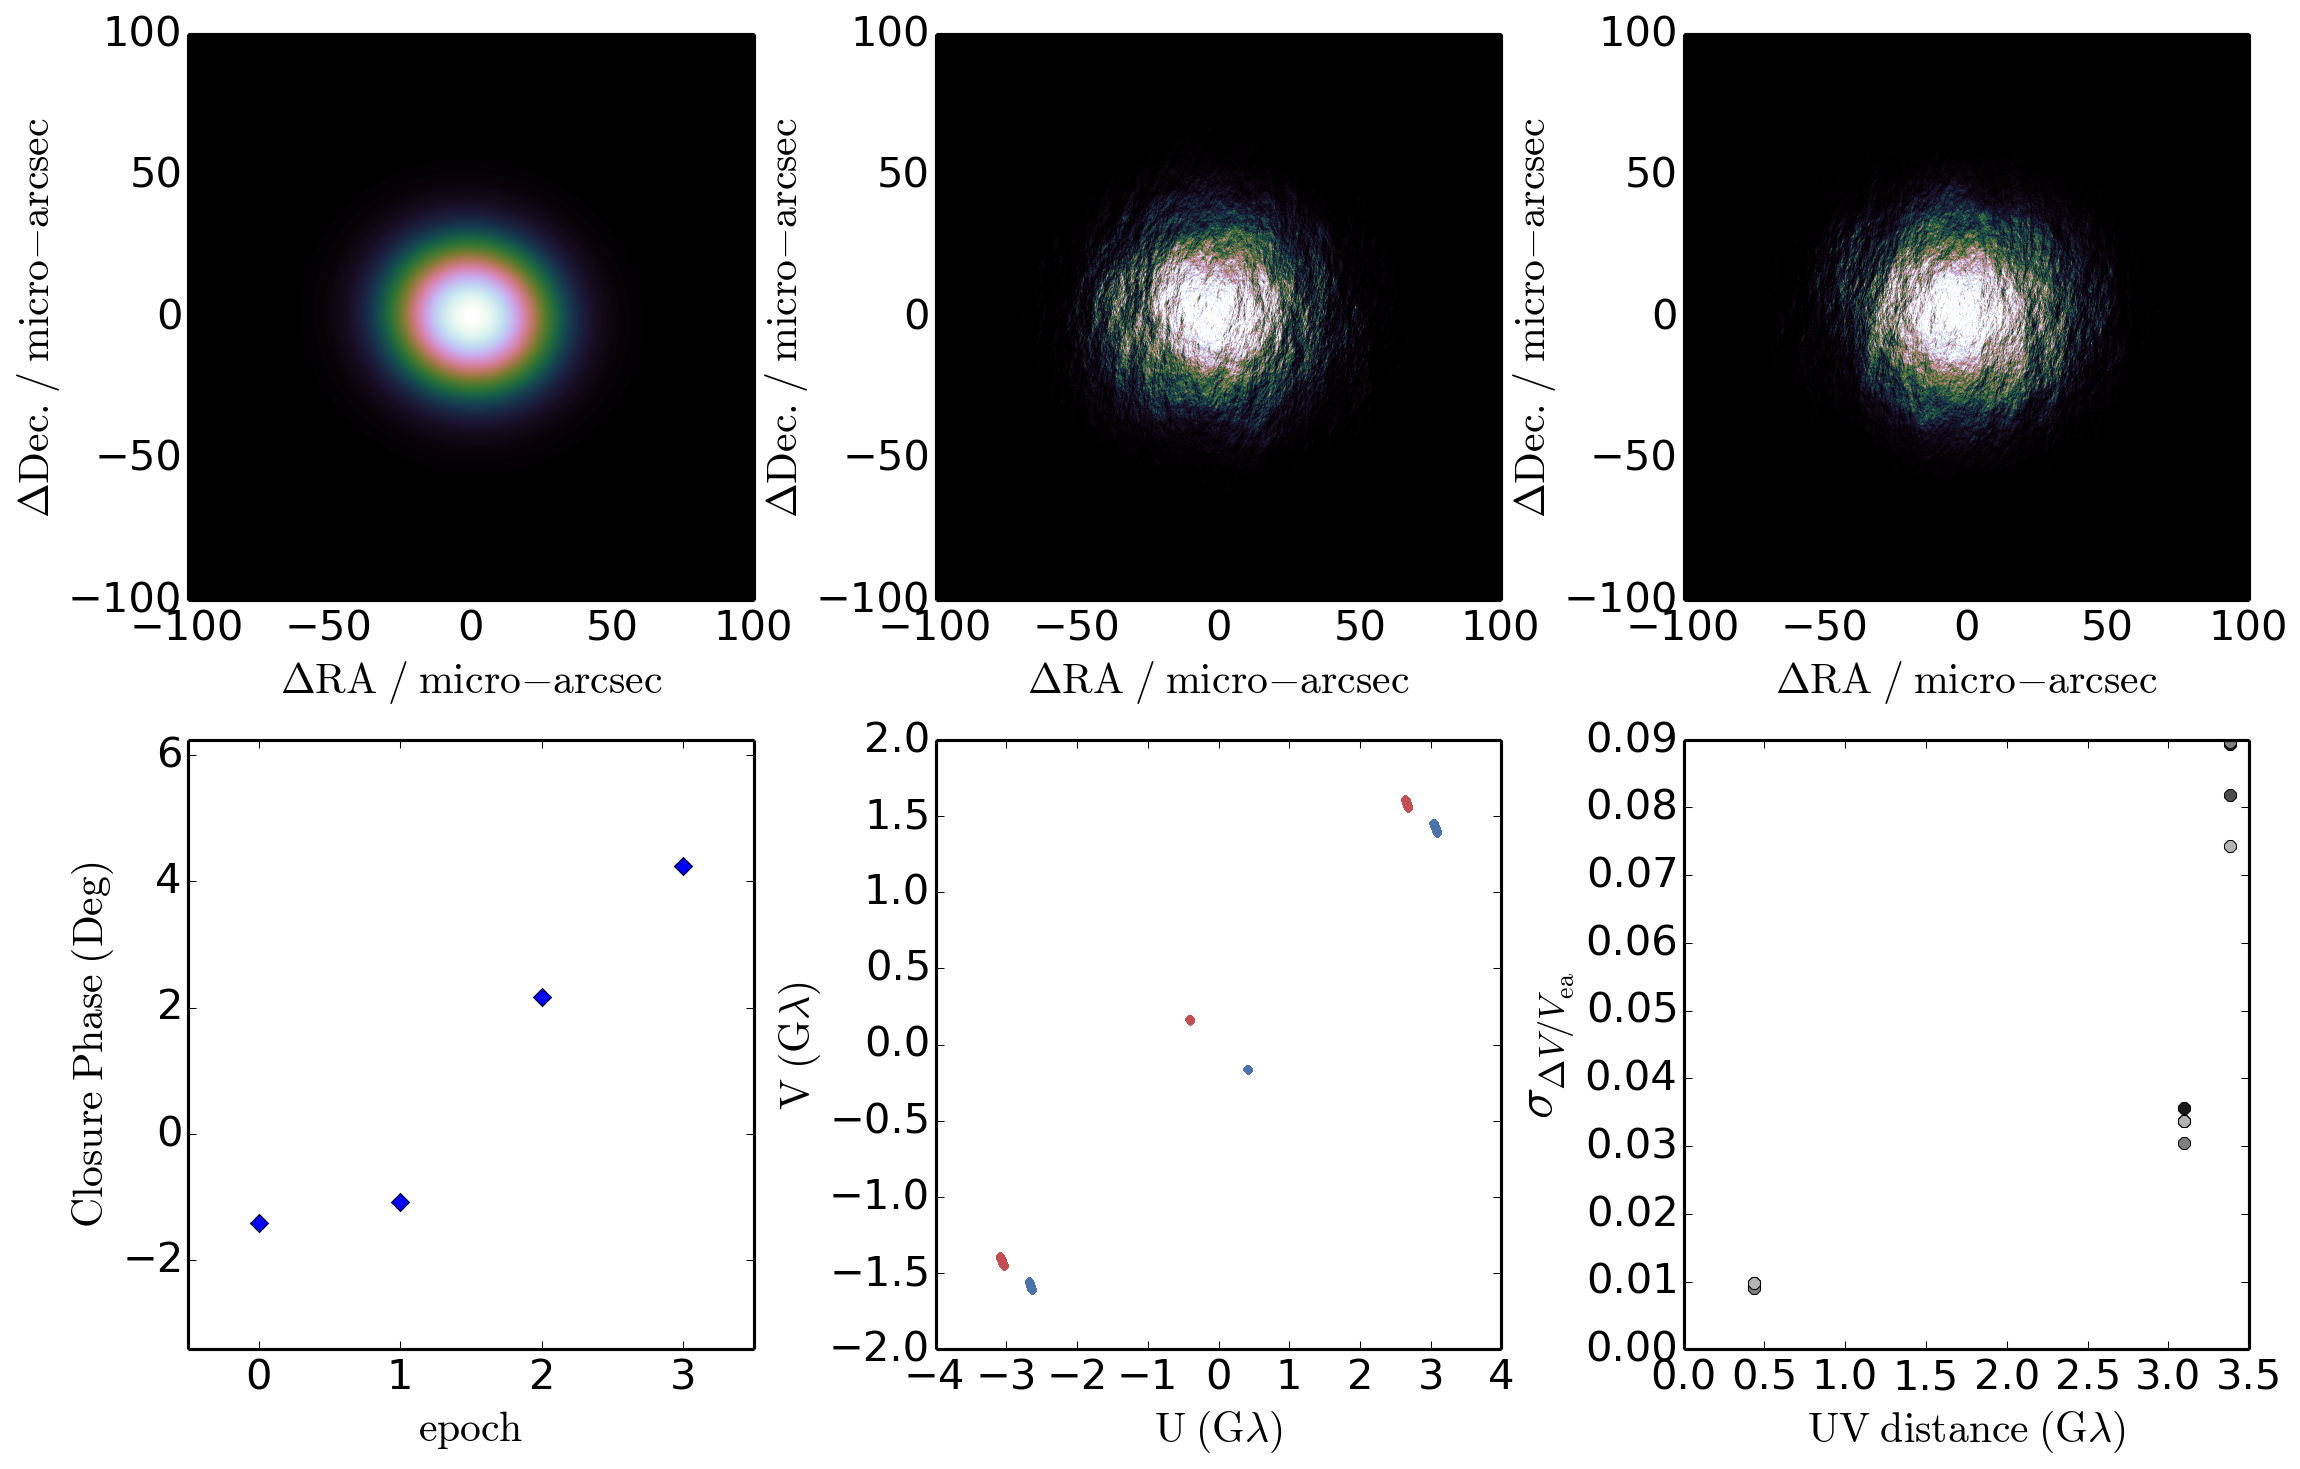
\includegraphics[width=\columnwidth]{Images/ism}
\caption{``An example simulation of ISM scattering towards Sgr~A$^{\star}$, observed with SMT-JCMT-CARMA.  The top panel, left to right, shows the original $\rm FWHM = 40$~$\mu$-arcsec Gaussian {\bf (top left)}, the simulated ISM scattered image on the first night {\bf (top middle)} and last night {\bf (top right)} of the observation, respectively.  The bottom panel, left to right,  shows the evolution of the 10 minute-averaged closure phase with epoch {\bf (bottom left)}, {\sl uv}-tracks for each night {\bf (bottom middle)} and the RMS fractional visibility amplitude differences $\sigma_{\Delta V /V_{\rm ea}}$ as a function of {\sl uv-}distance {\bf (bottom right)}. $ \Delta V= (|V_{\rm a}|-|V_{\rm ea}|)$, where $|V_{\rm a}|$ and |$|V_{\rm ea}|$ are the simulated average and ensemble average visibility amplitudes respectively. Variations from the ensemble-average flux on the shortest baselines reveal total flux modulation while flux variations on longer baselines and non-zero closure phases track the fluctuations in substructure.''(Image and caption reproduced from \citet{Blecher_2016}) \label{ISM_sequence}%
}
\end{figure}

\subsubsection{Atmospheric transmission and scattering}

As described in section~\ref{sec:trop_imp}, the implementation of the tropospheric module is separated into mean and turbulent components. For the mean atmosphere, we simulate opacity, sky brightness temperature and time delay as a function of site weather, elevation angle and frequency. The most important climate parameters are precipitable water vapour column depth, ground temperature and ground pressure. In the turbulent module we simulate Guassian fluctuations in the time delay arriving at each station, the variance of which is based on Kolmogorov turbulence.

%Opacity + Brightness temperature
The first atmospheric result we present are characteristic mean opacities and sky brightness temperatures for ALMA, the Submillimeter Array (SMA) and the South Pole Telescope (SPT) at 230~GHz, shown in Fig.~\ref{fig:mean_atm}. These sites were chosen as they are all considered excellent sites for sub-mm astronomy and form an essential part of the EHT. The PWV ranges used were taken from the 25th and 75th percentile data shown in \citet{Lane_1998} and is in good agreement with the measured opacities. 


\begin{figure}[h!]
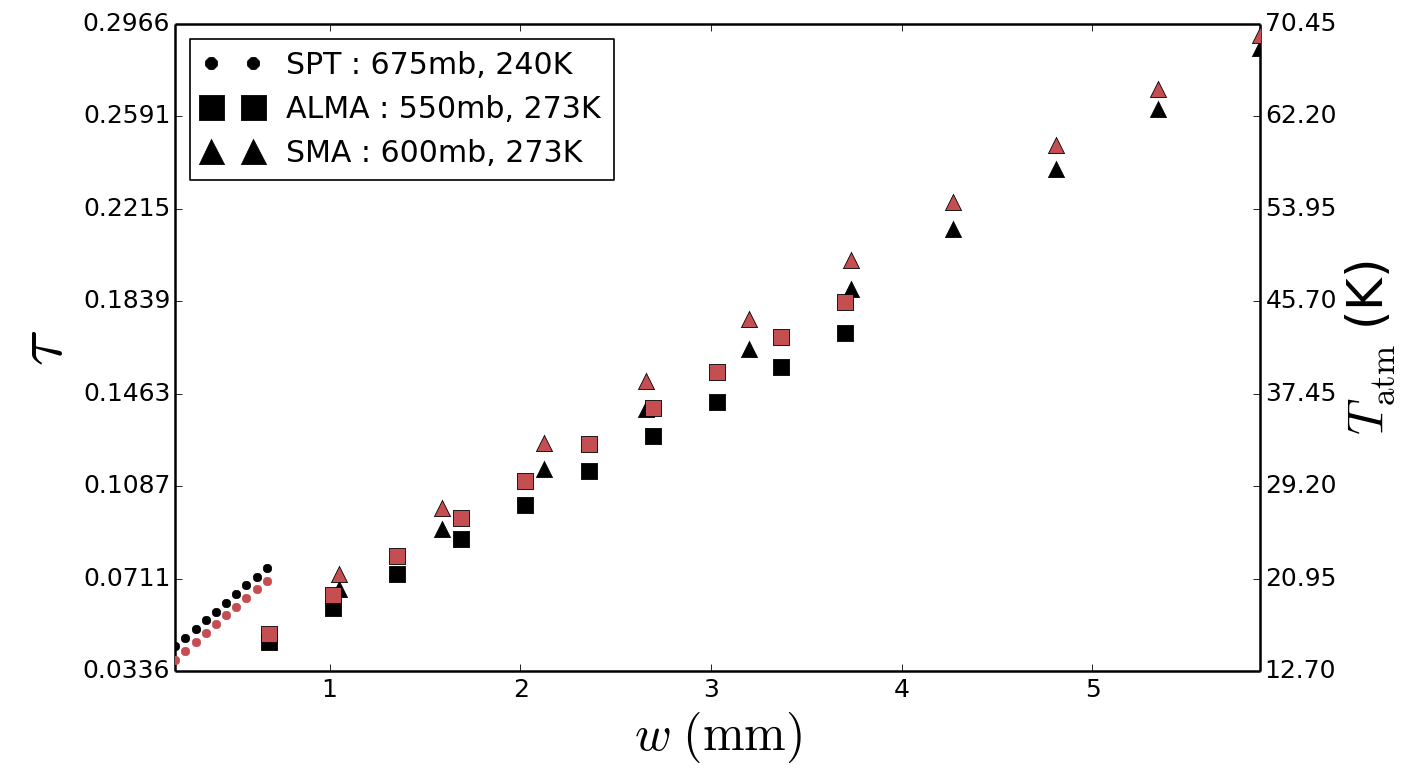
\includegraphics[width=1.\columnwidth]{Images/opacity}
\caption{``Simulated mean opacity (black) and sky brightness temperature (red) at $\nu =230$~GHz  for three typical ground pressures and temperatures over a typical PWV range \citep{Lane_1998} which approximately represent the sites of SPT (dots), ALMA (squares) and SMA (triangles). The legend shows the estimated input ground (pressure, temperature) parameters for each site.''(Image and caption reproduced from \citet{Blecher_2016})\label{fig:mean_atm}%
}
\end{figure}


Immediately apparent is that the opacity and brightness temperature both exhibit linear relationships with respect to PWV content and are proportional to ground pressure and inversely proportional to the ground temperature. It is also clear that SPT has far less opacity, and a lower sky brightness than ALMA and the SMA which are fairly similar. A comparison of the thermal temperature of the receiver (ALMA$\sim17$~K,  SMA$\sim711$~K, SPT$\sim 255$~K)\footnote{Values taken from http://www.eventhorizontelescope.org/proposal.html} reveals that for SPT and SMA the thermal noise contribution from the receiver is approximately an order of magnitude higher than atmospheric temperature however these values are comparable for ALMA, potentially limiting its sensitivity. 


%Turbulent and mean delay
Of vital importance to an interferometric site is the atmospheric stability. The effects of atmospheric transmission and scattering on delay and delay rate is shown in Fig.~\ref{delay_plots}. The total delay is made up of both mean turbulent components an example of the total and turbulent delays towards Sgr~A* is shown for SMA and ALMA. 


\begin{figure}[h!]
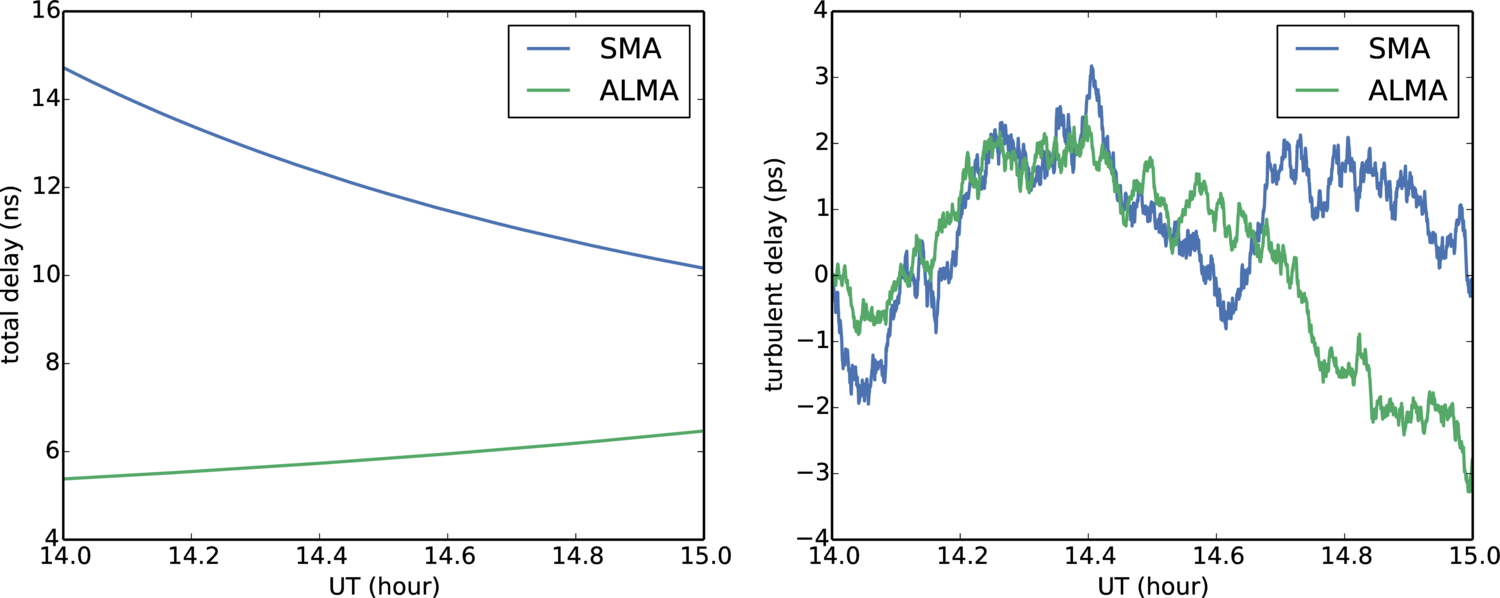
\includegraphics[width=\columnwidth]{Images/delays}
\caption{``Simulation of the total delay (left) and the turbulent atmospheric delay (right) for SMA (blue) and ALMA (green) sites towards Sgr~A$^\star$. Ground pressures and temperatures are the same as Fig.~\ref{fig:mean_atm}, precipitable water vapour above each station is set to $w=2$~mm, and the instantaneous zenith coherence time is set $T_0=10$~s for both stations. Note that all tropospheric parameters are, however, independently set. The conversion from time delay to phase at 230~GHz is $1$~rad~$=0.7$~ps.''(Image and caption reproduced from \citet{Blecher_2016})\label{delay_plots}%
}
\end{figure}


We see that the turbulent component is typically 3-4 orders of magnitude lower than the mean delay.

%Trop images
\begin{quotation}
``We now investigate the effect of the tropospheric module on image quality for various levels of calibration accuracy. We simulate the simple scenario of a sky model that consists of a 2.4~Jy point source at the phase centre, which is an approximate EHT-measured flux density of Sgr~A$^\star$ at 230~GHz. We assume a zenith phase coherence time of $t_0=10$~s above each station (however, each stations PWV can be independently simulated). We approximate the effect of imperfect calibration by adding a small fraction of the turbulent phase noise. For this example, we do not include the mean delay component, assuming it to be perfectly corrected for during the calibration. Imaging [is performed] using the two dimensional inverse fast Fourier transform''\\
\citep{Blecher_2016}
\end{quotation}

%Trop images
\begin{figure}[h!]
\includegraphics[width=\columnwidth]{Images/trop_images}
\caption{``The effect of residual troposphere phase noise on interferometric images of a point source observed for 12 hours at 230~GHz with 4~GHz bandwidth with the following array : SPT, ALMA, SMA, SMT, LMT and JCMT, assuming the same SEFDs as \protect\citet{Lu_2014} and an elevation limit of 15$^\circ$. For simplicity the weather parameters at each station were set to: coherence time $t_{\rm 0}=10$~sec; PWV depth $w=1$~mm; ground pressure $P=600$~mb; ground temperature $T =273$~K. {\bf Top left:} interferometric map with thermal noise only. {\bf Top right:} atmospheric attenuation and sky noise (due to non-zero opacity) with 1\% of the turbulent phase noise added. {\bf Bottom left:} as previous but with 3\% of turbulent phase contribution. {\bf Bottom right:} as previous but with 6\% turbulent phase contribution. The fractional turbulent phase contributions are illustrative of the effect of fringe-fitting errors. The black crosshairs indicate the original source position. ''(Image and caption reproduced from \citet{Blecher_2016}) \label{fig:trop_images}%
}
\end{figure}


We note a rapid attenuation in the original peak, central flux due to incoherent averaging. Specifically the flux central peak component is reduced to $76.5\%$ (attenuation only - not shown in plot), $75.1\%$ (1\% turbulence), 65.5\% (2\% turbulence) and  40.5\% (3\% turbulence). In the case of 3\% turbulence the lower artifact becomes brighter than the original source (44.5\%). 


There are also slight offsets in the source centroid as shown by progressive movement away from the black crosshairs. However this is quite a minor effect ($5.6\ \micro$-arcsec) at 3\% turbulence. 

Also interesting to note is the distortion of the interferometric artifacts presence of spurious imaging artefacts - when attempts to try clean don't work ! this messes with the subtraction of the PSF. PSF effects are distorted by turbulent atmosphere. Self-cal could make this worse.


There was no evidence of blurring ('seeing') or a loss of resolution. This would result if the decoherence is considered as a function of baseline length, longer baseline would be more decoherent and their visibilities are effectively downweighted. For the EHT as different stations would experience independent different turbulent intensities, the baseline length will not be correlated with the magnitude of the seeing. But as we've seen this does still distort the image which could lead to uncharacteristic feature extraction.

%Incoherent closure phases.. This section is needed to link up to the discussion on closure phase uncertainty in the mm-VLBI section. Yep worth mentioning. but leave this 

%NON-CLOSING ERRORS
%Non-closing errors due to incoherent averaging - "no conjugates for triples" - possibly comes down to how one defines SNR. In the definition used in the literature we followed, they assumed only gaussian noise, which was not the case..A better definition would be to look at the distribution of a number of samples 
%maybe just a mention of how the closure phase uncertainty could change.

\subsubsection{Pointing}

\begin{quotation}
``We investigate the effect of pointing errors on the 50~m (i.e. fully illuminated) Large Millimeter Array (LMT) dish configured in an eight station VLBI array. The LMT has been measured to have an absolute pointing accuracy of $\sigma_{\rm abs} = 1-3$~arcsec, where smaller offsets occur when observing sources closer to zenith, and a tracking pointing accuracy $\sigma_{\rm track} < 1$~arcsec\footnote{http://www.lmtgtm.org/telescope/telescope-description/}. We investigate the observational effect of these errors through three different pointing error models which explore different instructive and plausible scenarios. The LMT has been singled out as this may well serve as a reference station for the EHT array given its sensitivity and central geographic location. The source used is a circular Gaussian of characteristic size $\Theta_{\rm src}=50$ $\mu$-arcsec, located at the phase centre. For this investigation, as long as $\Theta_{\rm src} \ll \theta_{\rm PB}$, the exact structure of the source is unimportant. We approximate the LMT beam profile using an analytic WSRT beam model (equation~\ref{eq:wsrt_beam}) with a factor of two increase in the beam factor $C$ to take into account the increased dish size.''\\
\citep{Blecher_2016}
\end{quotation}

[!! TO check C - is this fWHM for LMT or WSRT?? - also repeated in imp]
where $C$ is a constant, with value $C \approx 130$~GHz$^{-1}$. Note that the power beam $EE^H$ becomes $\cos^6$, resulting in a $\rm{FWHM} = 6.5 $~arcsec at 230 GHz. 


We make use of the RMS fractional visibility amplitude error $\sigma_{\Delta V/V_0}$, where $V_{\rm PE}$ and $V_{0}$ are the visibility amplitudes with and without pointing errors respectively, and  $\Delta V = V_{\rm PE} - V_{0}$ . In Fig.~\ref{fig:pointing}, $\sigma_{\Delta V/V_0}$ is plotted against pointing error $\rho$ over the range $0 \le \rho \le 4.5$~arcsec.

In the first case we assume a \emph{constant} pointing error. This simulation is meant to be instructive as to the typical amplitude error in the simplest possible scenario.

''
[to be merged with the previous quotation]
In this simulation, we only consider LMT pointing errors due to its narrow primary beam and potential to be used as a reference station. However, the capability to simulate independent pointing errors for each station is available. In the case of a phased array, a pointing error simulation could be used to investigate the contribution of the pointing error to a variable phasing efficiency, which can be reasonably approximated by a scalar Jones matrix.''
''
\begin{figure}[h!]
\includegraphics[width=\columnwidth]{Images/point_Crop}
\caption{``RMS relative amplitude error induced by pointing error with the 50~m (i.e. fully illuminated) LMT antenna as a function of pointing error offset $\rho$ at 230~GHz. We assume that these errors are degenerate or non-separable from the self-calibration/fringe-fitting model used. See text for the description of the three models used. This simulation capability enables constraints on the magnitude of pointing-induced errors given a particular pointing calibration strategy.''(Image and caption reproduced from \citet{Blecher_2016})\label{fig:pointing}%
}
\end{figure}

\begin{quotation}
``Visibility amplitude errors due to antenna pointing error has been investigated for the $50$~m  LMT dish operating at $230$~GHz. In Fig.~\ref{fig:pointing}, we show that pointing errors associated with frequent phase centre switching (stochastic variability) could introduce a RMS fractional amplitude error $\sigma_{\Delta V/V_0} \sim 0.1 - 0.4$ for an absolute pointing accuracy  $\sigma_{\rm abs} \sim 1-3$~arcsec. In contrast, tracking errors are less problematic with $\sigma_{\Delta V/V_0} \le 0.05$ for a tracking accuracy  $\sigma_{\rm track}<1$~arcsec. The case of a constant error pointing model is comparable to that of the `slow variability' case. If the gain error is non-separable from the calibration model used, it could be interpreted as intrinsic variability, substructure and/or increased noise. If unaccounted for, this effect has the potential to limit the dynamic range of mm-VLBI images. Further tests to constrain the pointing uncertainties of EHT stations will lead to more accurate interferometric simulations and hence the overall impact on black hole shadow parameter estimation. Here we demonstrate the capability to incorporate a range of plausible pointing error effects into a full simulation pipeline. For future observations at 345~GHz, these effects will be even more pronounced, given the narrower primary beam.

[..]
\\
\citep{Blecher_2016}
\end{quotation}


%\subsubsection{Performance?}
%Performance/speed

%\section{Fringe-fitting test}
%leave until done
%First we fringe fit and image a stationary point source and compare to the result in Fig.~\ref{fig:trop_images}. 
% In an upcoming paper, we perform a systematic exploration of the turbulent tropospheric effects on the accuracy of fringe-fitting algorithms/strategies, through use of an automated calibration procedure and including the added complexity of a time-variable source.


%additional discussion

% Include this q&a -> not sure which chapter is best though...maybe intro and theory to prevent a reader sitting with the question for so long
-The authors list a couple of observational challenges and claim that pointing errors, as they have implemented in the simulator, are non-negligible instrumental errors. I think there are more “subtle” instrumental effects that need to be taken into account or should be pointed out to give a full story to the reader. Without an estimate of these effects, I am not sure if you can simply ignore them. A related question: does the simulator have a different treatment of instrumental model for single dish and phased array?

>>True, there are many additional potential sources of error (e.g. clock errors, bandpass, polarisation leakage, phasing errors, quantisation, correlator model etc.). The point of this first paper is to demonstrate the mm-VLBI framework that enables more sophisticated interferometric simulations. As such, we have focused on capabilties not present in other mm-VLBI simulations and represent different Jones Matrix implmentations (i.e. the troposphere, ISM and antenna pointing errors). These also represent amongst the most challenging signal corruptions to implement. As we state in the manuscript, the MeqSilhouette framework, rooted in the Measurement Equation formalism, enables any arbitary error to be incorporated as a Jones Matrix (e.g. correlator model error is a simple scale matrix [e^-\phi, 0, e^-\phi, 0]). Our intention here is to demonstrate some of the key features of MeqSilhouette and its potential to provide realistic mm-VLBI simulations for systmatic studies that will be reported in future papers. At present, we use the same model for a single dish and phased array, we have now included a discussion on the implication for phased arrays in both the turbulent troposphere pointing error sections.


%Maybe jnust provide a brief note in the implementation
-MeqSilhouette is a VLBI simulator in the first place. The central components described in the paper focus mainly on the signal corruption, but without giving details on the visibility generation and sampling. Given the ultra-wide-band VLBI systems for future observations, are there any systematic uncertainties that a simulator primarily designed for low frequency facilities could bring in?

>>Visibility generation and sampling is performed through the evaluation of the Fourier Transform at every UVW point in the data. This has been added to the text. Ultra-wide bandwidth observations would require sampling at the appropriate frequency and time resolution in order to avoid smearing effects. MeqTrees can generate visibilities at any arbitrary time and frequency resolution and so we do not anticipate this to be a problem, provided the appropriate choices are made to accurately image the processed field-of-view.



% move to that paragraph in the intro
p.2, second last para. The previous simulation work used closure phase as a primary observable, which is in principle immune to station-based phase errors. So I think a nearly perfect phase calibration is well justified, although amplitudes may suffer from systematic calibration errors, which the current work do not consider either for most effects. What is the reason to introduce a variable smoothing kernel? Do you mean refractive substructure?

>>The increase in sensitivity and number of EHT stations for the observing run in 2017 marks a shift towards first imaging attempts. Therefore, while previous simulations may have been justified in perfect phase calibration due to a closure quantity only analysis, we now need to move towards a more complex framework to incorporate the relevant corruptions for imaging. Yes, up until now we have considered only several amplitude systematics (pointing error, phase incoherence due to tropospheric turbulence, non-zero atmospheric opacity and emission) but this can be expanded upon in future (specifically a paper on fringe-fitting accuracy and systematics for a range of tropospheric conditions).
Yes we mean refractive substructure. This has been clarified in the text. " [they] assume .. only Gaussian convolution to simulate ISM scattering" 